\documentclass[12pt]{article}
\usepackage[spanish, english, es-tabla]{babel}
\usepackage[utf8]{inputenc}
\usepackage{amsmath,amssymb}
\usepackage{graphicx}
\usepackage{gensymb}
\usepackage{outlines}
\usepackage[export]{adjustbox}
\usepackage{adjustbox}
\usepackage{multicol}
\usepackage{lipsum}
\parskip 1ex

\usepackage{eurosym}

% add code
\usepackage{listings}

\usepackage{array}

% text font 

\usepackage{courier}

%\usepackage{fontspec}

\usepackage[dvipsnames]{xcolor}

\usepackage{hyperref}
\usepackage{subcaption}
\usepackage[left = 2cm, right = 2cm, bottom = 2cm, top = 3cm]{geometry}

\hypersetup{
	colorlinks=true,
	linkcolor=black,
	%filecolor=magenta,      
	urlcolor=cyan,
}

\hypersetup{
	pdftitle= {Diseño y automatización de un sistema de alimentación OpenSource para animales a través de la tecnología LoRa},
	pdfauthor = {Lucía Francoso Fernández},
	pdfsubject = {Electrónica y comunicaciones móviles},
	pdfkeywords = {Arduino, LoRa, automatización, LoRaWAN, punto a punto, OpenSource}
}

% define color for C code (Anexos)

\definecolor{codegreen}{rgb}{0,0.6,0}
\definecolor{codegray}{rgb}{0.5,0.5,0.5}
\definecolor{codepurple}{rgb}{0.58,0,0.82}
\definecolor{backcolour}{rgb}{0.95,0.95,0.92}

\lstdefinestyle{mystyle}{
	backgroundcolor=\color{backcolour},   
	commentstyle=\color{codegreen},
	keywordstyle=\color{magenta},
	numberstyle=\tiny\color{codegray},
	stringstyle=\color{codepurple},
	basicstyle=\ttfamily\footnotesize,
	breakatwhitespace=false,         
	breaklines=true,                 
	captionpos=b,                    
	keepspaces=true,                 
	numbers=left,                    
	numbersep=5pt,                  
	showspaces=false,                
	showstringspaces=false,
	showtabs=false,                  
	tabsize=2
}

\lstset{style=mystyle}

% https://tex.stackexchange.com/questions/60209/how-to-add-an-extra-level-of-sections-with-headings-below-subsubsection
\newcommand{\subsubsubsection}[1]{\paragraph{#1}\mbox{}\\}
\setcounter{secnumdepth}{4}
\setcounter{tocdepth}{4}

\begin{document}
	\selectlanguage{spanish}
	
	%\thispagestyle{empty}
	
	
	
	%\pagebreak
	
	\thispagestyle{empty}
	
	\newgeometry{left=0.01cm,bottom=0.01cm, top=0.01cm}
	
	%width=0.3\textwidth,
	
	%\begin{figure}[h!]
	%	
\includegraphics[height=\textheight,left]{img/banda_etsit_90.png}
	
	%	\end{figure}
	
	\begin{minipage}{0.2\textwidth}
		
\includegraphics[height=\textheight,left]{img_comp/banda_etsit_90.png}
	\end{minipage}
	\centerline{\begin{minipage}[t][7cm][b]{0.5\textwidth}
			%	\textbf{UNIVERSIDAD POLITÉCNICA DE} \\
			
			%	\textbf{CARTAGENA}\\
			
			\vspace{2cm}
			
			\title{\textbf{Automatización y control de bebederos automáticos para especies animales usando LoRa: }\\
				
			\vspace{1cm}
			
			\textit{Documentación de la página web} 
			}
			
			\maketitle
			
			\vspace{1cm}
				
			\hspace{1.5cm} \textbf{TRABAJO FIN DE GRADO} \\
			
			\vspace{0.5cm}
			
			\hspace{1.3cm} Grado en Ingeniería en Sistemas  de\\
			
			\vspace{0.01cm}
			
			\hspace{2.7cm} Telecomunicaciones \\
			
			\vspace{1cm}
			
			\textbf{Autora:}\author{ Lucía Francoso Fernández}\\
			
			\textbf{Tutor:} Juan Pascual García
	\end{minipage}}
	
	
	\restoregeometry
	
	\pagebreak

	\tableofcontents
	
	\pagebreak
	
	\listoffigures
	\addcontentsline{toc}{section}{Índice de figuras}
	
	\pagebreak
	
	\listoftables
	\addcontentsline{toc}{section}{Índice de tablas}
	
	\pagebreak
	
	\section{Introducción}
	
	\noindent En este documento se recoge una pequeña documentación sobre la página web \textit{Open Pet Feeder}, una web creada bajo el marco del Trabajo Fin de Grado especificado en el título del presente, \textit{Automatización y control de bebederos automáticos para especies animales usando LoRa}. Es una parte fundamental para la consecución de ciertos objetivos del proyecto, entre ellos, la monitorización de la estación que se situará en el refugio de Patitas Unidas Los Alcázares, desde cualquier dispositivo y desde cualquier sitio (dentro o fuera de la red local de la estación donde se sitúa el servidor que almacena la web).\\
	
	\noindent Comprende explicaciones sobre el funcionamiento de la misma, así como explicaciones sobre la creación de la web. Para una introducción a la página web más visual, se incluyen capturas bajo diferentes situaciones.\\
	
	\section{Apariencia de la web}
	
	\begin{figure}[h!]
		\begin{center}
			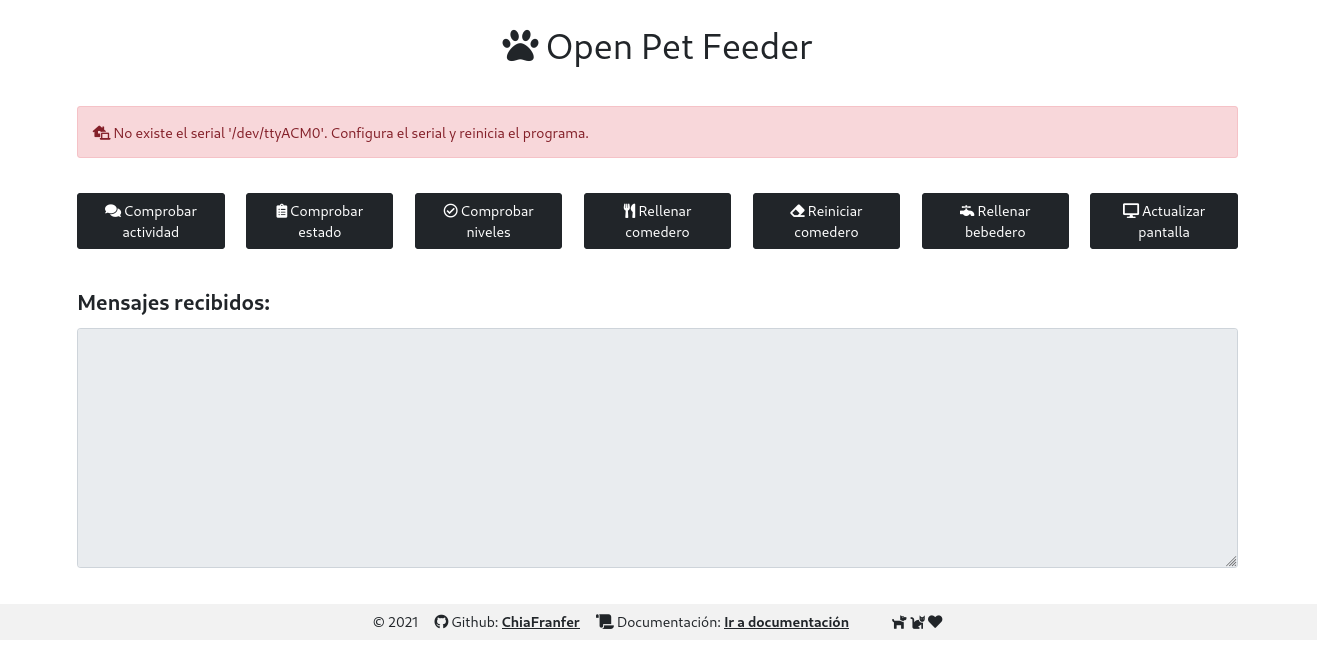
\includegraphics[width=1\textwidth]{img_comp/captura_web_1.png}
			\caption{Captura de la web \textit{Open Pet Feeder}, donde se muestra el mensaje de error al no detectar la conexión serial con el arduino.}
			\label{captura web 1}
		\end{center}
	\end{figure}

	\pagebreak
	
	\begin{figure}[h!]
		\begin{center}
			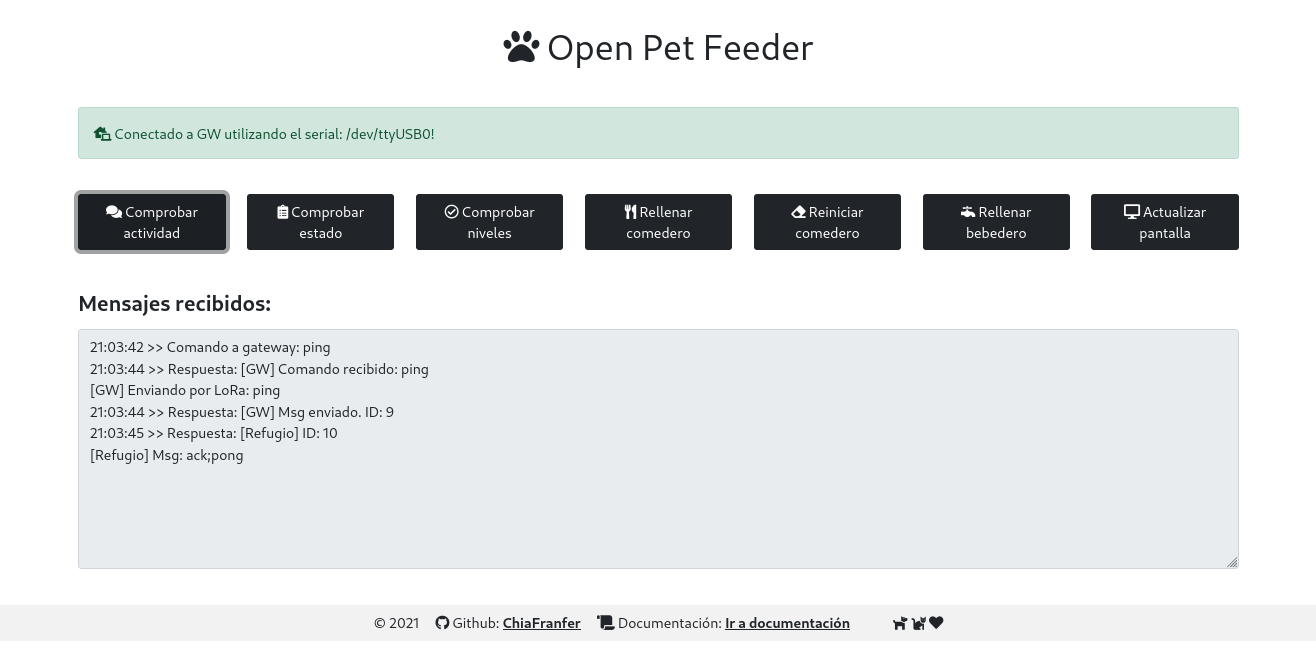
\includegraphics[width=1\textwidth]{img_comp/captura_web_2.png}
			\caption{Captura de la web \textit{Open Pet Feeder}, donde se muestra en la consola la interacción entre estación del campo y estación del refugio a través del comando \textit{ping} (botón \textit{Comprobar actividad}).}
			\label{captura web 2}
		\end{center}
	\end{figure}
	
	\pagebreak
	
	\begin{figure}[h!]
		\begin{center}
			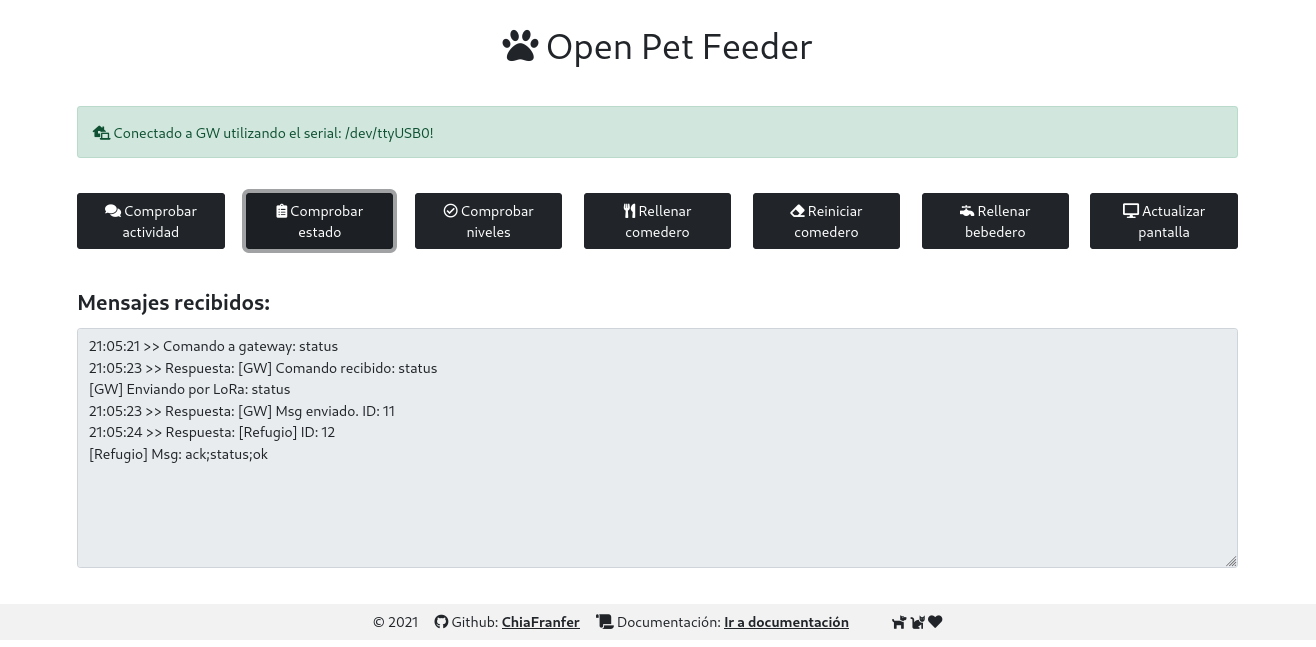
\includegraphics[width=1\textwidth]{img_comp/captura_web_3.png}
			\caption{Captura de la web \textit{Open Pet Feeder}, donde se muestra en la consola la interacción entre estación del campo y estación del refugio a través del comando \textit{status} (botón \textit{Comprobar estado}).}
			\label{captura web 3}
		\end{center}
	\end{figure}

	\pagebreak
	
	\begin{figure}[h!]
		\begin{center}
			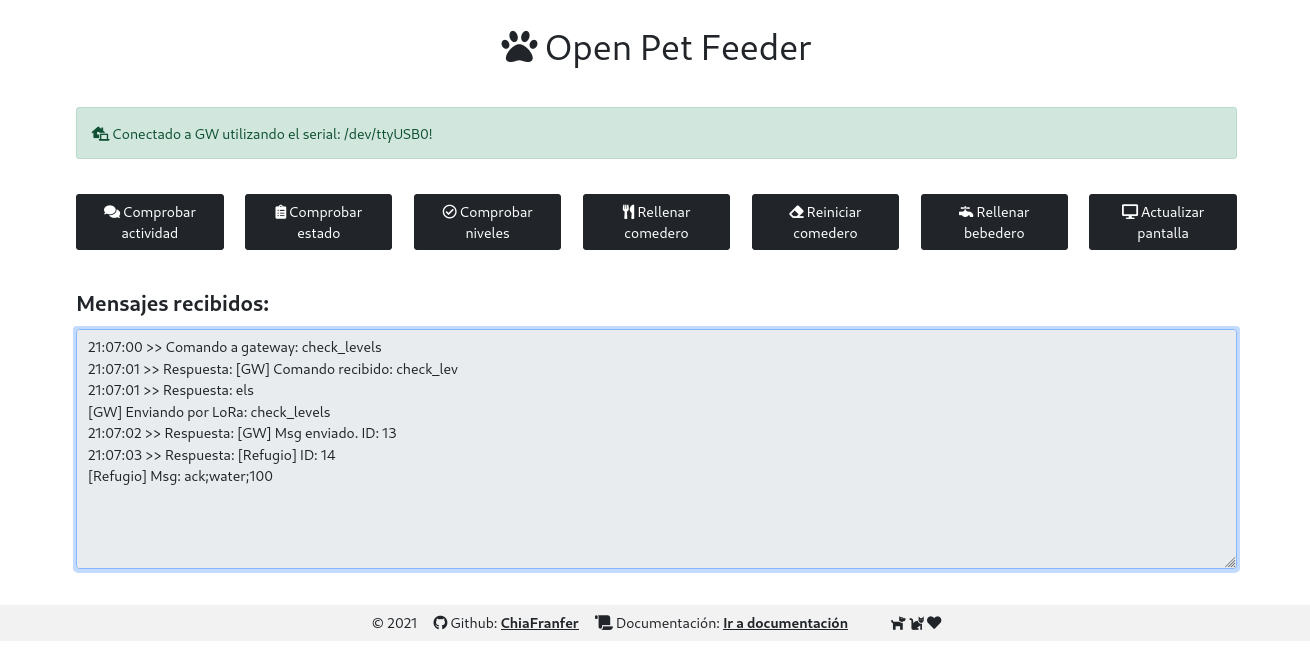
\includegraphics[width=1\textwidth]{img_comp/captura_web_4.png}
			\caption{Captura de la web \textit{Open Pet Feeder}, donde se muestra en la consola la interacción entre estación del campo y estación del refugio a través del comando \textit{check\_levels} (botón \textit{Comprobar niveles}).}
			\label{captura web 4}
		\end{center}
	\end{figure}

	\pagebreak
	
	\begin{figure}[h!]
		\begin{center}
			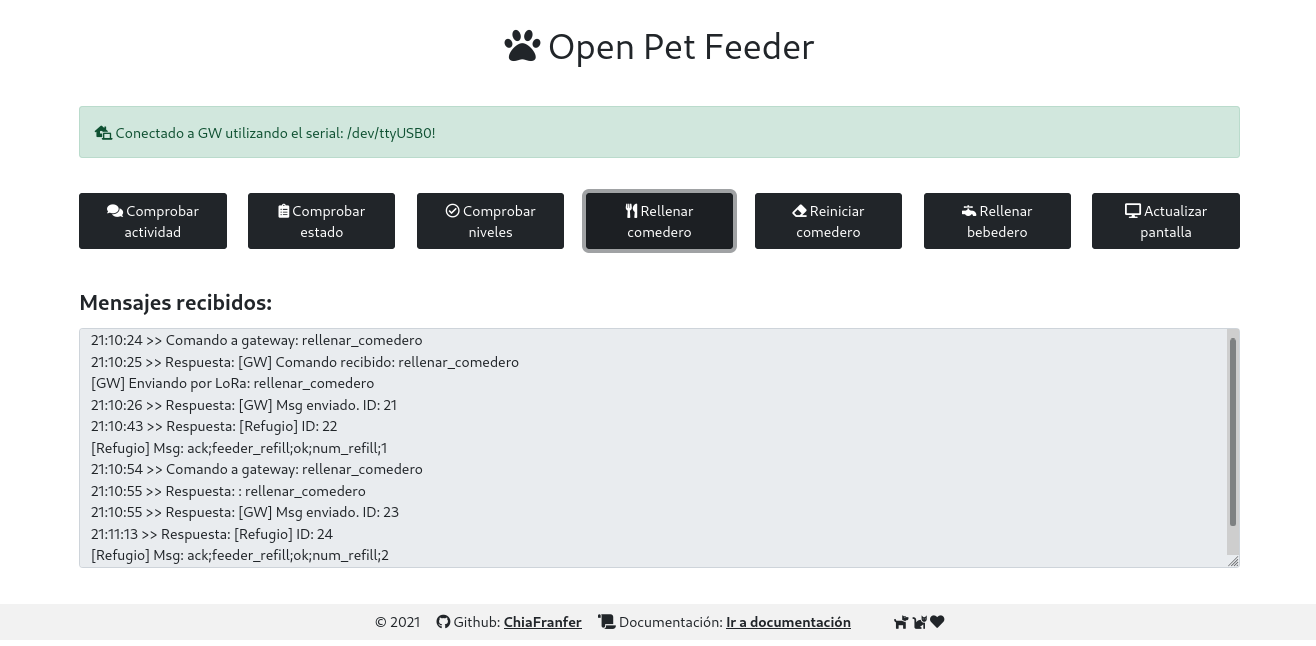
\includegraphics[width=1\textwidth]{img_comp/captura_web_5.png}
			\caption{Captura de la web \textit{Open Pet Feeder}, donde se muestra en la consola la interacción entre estación del campo y estación del refugio a través del comando \textit{rellenar\_comedero} (botón \textit{Rellenar comedero}).}
			\label{captura web 5}
		\end{center}
	\end{figure}

	\pagebreak
	
	\begin{figure}[h!]
		\begin{center}
			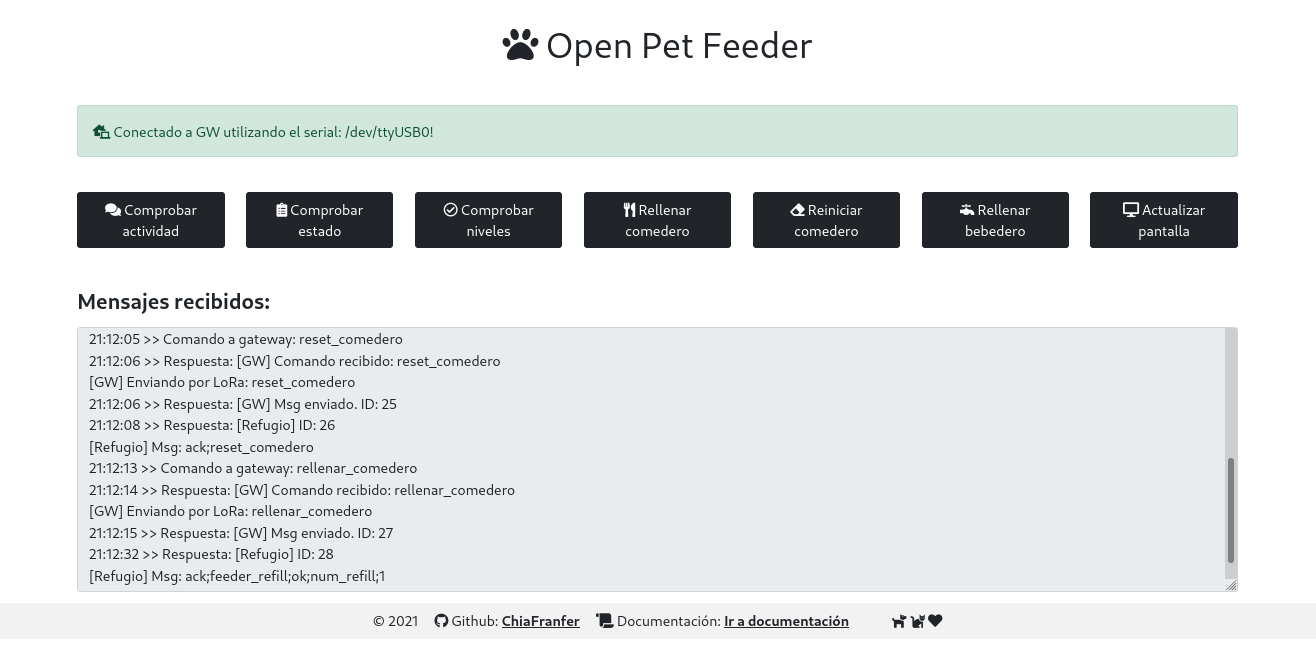
\includegraphics[width=1\textwidth]{img_comp/captura_web_6.png}
			\caption{Captura de la web \textit{Open Pet Feeder}, donde se muestra en la consola la interacción entre estación del campo y estación del refugio a través del comando \textit{reset\_comedero} (botón \textit{Reiniciar comedero}).}
			\label{captura web 6}
		\end{center}
	\end{figure}

	\pagebreak
	
	\begin{figure}[h!]
		\begin{center}
			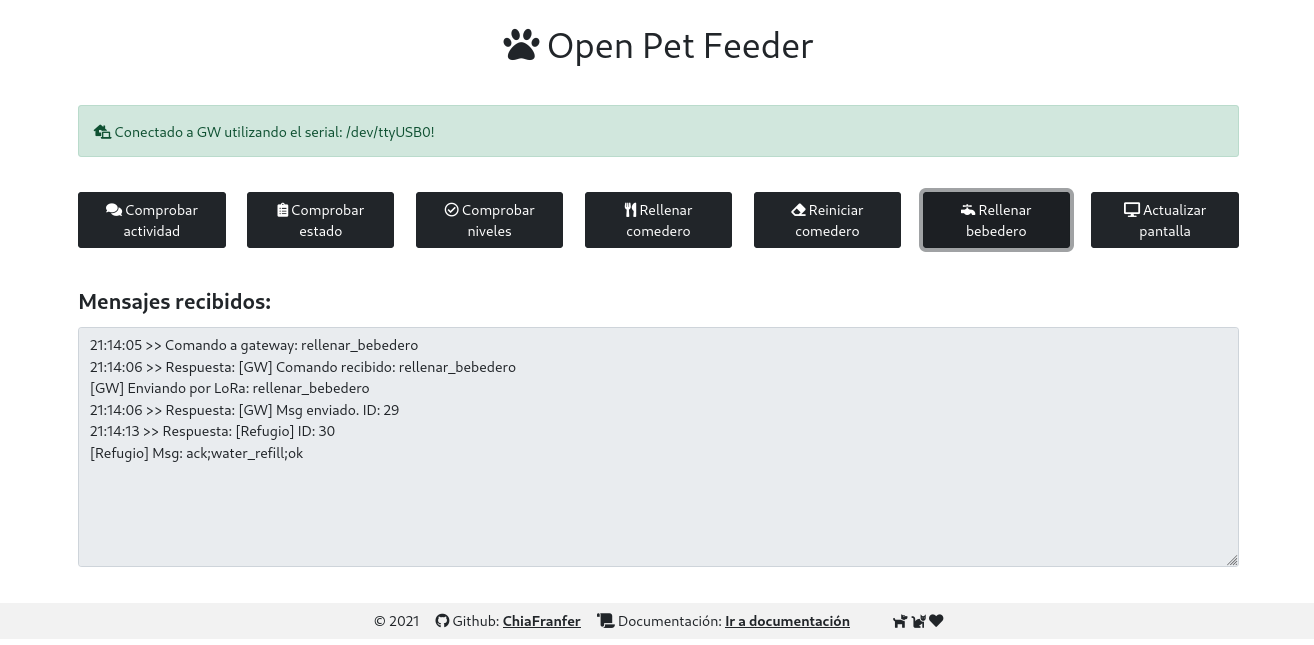
\includegraphics[width=1\textwidth]{img_comp/captura_web_7.png}
			\caption{Captura de la web \textit{Open Pet Feeder}, donde se muestra en la consola la interacción entre estación del campo y estación del refugio a través del comando \textit{rellenar\_bebedero} (botón \textit{Rellenar bebedero}).}
			\label{captura web 7}
		\end{center}
	\end{figure}
	
	\noindent El botón \textit{Actualizar pantalla} (comando asociado \textit{update\_oled}) no realiza la función que describe su nombre, ya que no se implementó a nivel arduino por ocupar más espacio del disponible en el arduino nano (la librería \textit{OLED} ocupa bastante espacio). Si se envía este comando, la estación del refugio devuelve un string con ``\textit{to do}'', indicando que hay que implementarlo.\\
	
	\pagebreak
	
	\section*{Anexo}
	\addcontentsline{toc}{section}{Anexo}
	\label{anexo: codigo}
	
	\noindent En este anexo, se incluye el código empleado para crear la web. \\
	
	\noindent \textit{\textbf{Aplicación web}}: \textit{app.py}\\
	
	\begin{lstlisting}[language=python]
import engineio
from flask import Flask, render_template
from flask_socketio import SocketIO
from flask_serial import Serial
from datetime import datetime

import json
import socketio
import os

app = Flask(__name__)

## Configuration Serial GW
serial_port = '/dev/ttyUSB0'                    # Modificar aqui el serial del Arduino, lo dice el IDE
app.config['SERIAL_PORT'] = serial_port
app.config['SERIAL_TIMEOUT'] = 0.1
app.config['SERIAL_BAUDRATE'] = 115200
app.config['SERIAL_BYTESIZE'] = 8
app.config['SERIAL_PARITY'] = 'N'
app.config['SERIAL_STOPBITS'] = 1

socketio = SocketIO(app, async_mode="gevent", ping_timeout=5, logger=False, engineio_logger=False)
ser = Serial(app)

#
#   Enpoints
#

# Endpoint home page
@app.route("/")
def index():
# Comprobamos que el serial existe
if os.path.exists(serial_port):
serial_exists = True
else:
serial_exists = False

return render_template("index.html", serial_port=serial_port, serial_exists=serial_exists)

# Endpoint documentation page
@app.route("/doc")
def doc():
return render_template("doc.html")

#
#   SocketIO
#

# Handler SocketIO [messages of web]
@socketio.on('send')
def handle_send(json_str):
data = json.loads(json_str)["message"]
print("Boton pulsado: {}".format(data))

# Enviamos por serial
try:
ser.on_send(data)
except Exception as ex:
print("Error on serial: {}".format(ex))

# Enviamos en el socket 'receive_message' [hacer en recepcion serial]
now = datetime.now()
msg = "{} >> Comando a gateway: {}".format(now.strftime("%H:%M:%S"), data)
socketio.emit("receive_message", data={"message":str(msg)})

#
#   Flask-Serial
#

# Handler incoming serial messages
@ser.on_message()
def handle_message(msg):
try:
print("receive message: {}".format(msg))
now = datetime.now()
msg = "{} >> Respuesta: {}".format(now.strftime("%H:%M:%S"), msg.decode("utf-8").strip('\n'))
print("Send socket msg: {}".format(msg))
socketio.emit("receive_message", data={"message":str(msg)})
except Exception as ex:
print(ex)

# Log thread serial
@ser.on_log()
def handle_logging(level, info):
print(level, info)

if __name__ == '__main__':
socketio.run(app, debug=False, log_output=True)
	\end{lstlisting}

	\noindent \textit{\textbf{Página principal de la web}}: \textit{index.html}\\
	
	\begin{lstlisting}[language=html]
<!doctype html>
<html lang="es">
<head>
<!-- Required meta tags -->
<meta charset="utf-8">
<meta name="viewport" content="width=device-width, initial-scale=1">
<link rel="icon" type="image/png" href="static/favicon.ico">

<!-- Bootstrap CSS -->
<link href="https://cdn.jsdelivr.net/npm/bootstrap@5.0.2/dist/css/bootstrap.min.css" rel="stylesheet" integrity="sha384-EVSTQN3/azprG1Anm3QDgpJLIm9Nao0Yz1ztcQTwFspd3yD65VohhpuuCOmLASjC" crossorigin="anonymous">
<link rel="stylesheet" href="https://cdnjs.cloudflare.com/ajax/libs/font-awesome/5.15.3/css/all.min.css" integrity="sha512-iBBXm8fW90+nuLcSKlbmrPcLa0OT92xO1BIsZ+ywDWZCvqsWgccV3gFoRBv0z+8dLJgyAHIhR35VZc2oM/gI1w==" crossorigin="anonymous" referrerpolicy="no-referrer" />
<script src="https://cdn.socket.io/3.1.3/socket.io.min.js" integrity="sha384-cPwlPLvBTa3sKAgddT6krw0cJat7egBga3DJepJyrLl4Q9/5WLra3rrnMcyTyOnh" crossorigin="anonymous"></script>
<script src="https://code.jquery.com/jquery-3.6.0.min.js" integrity="sha256-/xUj+3OJU5yExlq6GSYGSHk7tPXikynS7ogEvDej/m4=" crossorigin="anonymous"></script>

<title>Open Pet Feeder</title>
</head>
<body>
<h1 style="text-align: center; margin-top: 2%;"><a href="/" style="text-decoration: none; color: inherit;"><i class="fas fa-paw"></i> Open Pet Feeder</a></h1>


<div class="container" style="margin-top: 3%;">

	<div class="alert alert-success" role="alert" style="margin-bottom: 3%;">
	<i class="fas fa-laptop-house"></i> Conectado a GW utilizando el serial: {{serial_port}}!
	</div>
	
		<div class="alert alert-danger" role="alert" style="margin-bottom: 3%;">
		<i class="fas fa-laptop-house"></i> No existe el serial '{{serial_port}}'. Configura el serial y reinicia el programa.
		</div>
		
			
			<div class="row" style="text-align: center;">
			<div class="col">
			<button type="button" class="btn btn-dark mt-1" id="send_ping" value="ping"><i class="fas fa-comments"></i>  Comprobar actividad</button>
			</div>
			<div class="col">
			<button type="button" class="btn btn-dark mt-1" id="send_status" value="status"><i class="fas fa-clipboard-list"></i>  Comprobar estado</button>
			</div>
			<div class="col">
			<button type="button" class="btn btn-dark mt-1" id="send_check_levels" value="check_levels"> <i class="far fa-check-circle"></i>  Comprobar niveles</button>
			</div>
			<div class="col">
			<button type="button" class="btn btn-dark mt-1" id="send_comedero" value="rellenar_comedero"><i class="fas fa-utensils"></i> Rellenar comedero</button>
			</div>
			<div class="col">
			<button type="button" class="btn btn-dark mt-1" id="send_reset_comedero" value="reset_comedero"><i class="fas fa-eraser"></i> Reiniciar comedero</button>
			</div>
			<div class="col">
			<button type="button" class="btn btn-dark mt-1" id="send_bebedero" value="rellenar_bebedero"><i class="fas fa-faucet"></i> Rellenar bebedero</button>
			</div>
			
			<div class="col">
			<button type="button" class="btn btn-dark mt-1" id="send_oled" value="update_oled"><i class="fas fa-desktop"></i> Actualizar pantalla</button>
			</div>
			</div>
			</div>
			
			<div class="container" style="margin-top: 3%;">
			<div class="console">
			<label class="form-label" for="receive"> <h4> <b>Mensajes recibidos:</b> </h4>  </label>
			<textarea readonly class="form-control" name="receive" id="receive" rows="8" style="width: 100%; height: auto;"></textarea>
			</div>
			</div>
			
			<!-- Footer -->
			<div class="footer fixed-bottom mt-4 py-4">
			<div class="text-center p-2" style="background-color: rgba(0, 0, 0, 0.05); margin-bottom: -1%;">
			C  2021  <i class="fab fa-github" style="margin-left: 1%;"></i> Github:
			<a class="text-reset fw-bold" href="https://github.com/ChiaFranfer">ChiaFranfer</a> 
			<i class="fas fa-scroll" style="margin-left: 1%;"></i> Documentacion: <a class="text-reset fw-bold" href="{{url_for('doc')}}"> Ir a documentacion</a>
			<i class="fas fa-dog" style="margin-left: 3%;"></i> <i class="fas fa-cat"></i> <i class="fas fa-heart"></i>
			</div>
			</div>
			
			<script src="https://cdn.jsdelivr.net/npm/bootstrap@5.0.2/dist/js/bootstrap.bundle.min.js" integrity="sha384-MrcW6ZMFYlzcLA8Nl+NtUVF0sA7MsXsP1UyJoMp4YLEuNSfAP+JcXn/tWtIaxVXM" crossorigin="anonymous"></script>
			<script type="text/javascript" charset="utf-8">
			$(document).ready(function() {
				var socket = io.connect('http://' + document.domain + ':' + location.port);
				
				$('#send_status').on('click', function() {
					var message = $(this)[0].value;
					console.log('Enviando: ' + message);
					var data = '{' + '"message": "' + message + '"}';
					socket.emit('send', data=data);
				});
				
				$('#send_ping').on('click', function() {
					var message = $(this)[0].value;
					console.log('Enviando: ' + message);
					var data = '{' + '"message": "' + message + '"}';
					socket.emit('send', data=data);
				});
				
				$('#send_reset_comedero').on('click', function() {
					var message = $(this)[0].value;
					console.log('Enviando: ' + message);
					var data = '{' + '"message": "' + message + '"}';
					socket.emit('send', data=data);
				});
				
				$('#send_comedero').on('click', function() {
					var message = $(this)[0].value;
					console.log('Enviando: ' + message);
					var data = '{' + '"message": "' + message + '"}';
					socket.emit('send', data=data);
				});
				
				$('#send_bebedero').on('click', function() {
					var message = $(this)[0].value;
					console.log('Enviando: ' + message);
					var data = '{' + '"message": "' + message + '"}';
					socket.emit('send', data=data);
				});
				
				$('#send_check_levels').on('click', function() {
					var message = $(this)[0].value;
					console.log('Enviando: ' + message);
					var data = '{' + '"message": "' + message + '"}';
					socket.emit('send', data=data);
				});
				
				$('#send_oled').on('click', function() {
					var message = $(this)[0].value;
					console.log('Enviando: ' + message);
					var data = '{' + '"message": "' + message + '"}';
					socket.emit('send', data=data);
				});
				
				socket.on('receive_message', function(data){
					console.log(data);
					var text = data['message'];
					var $textarea = $('#receive');
					$textarea.val($textarea.val() + text + '\n');
					$textarea.scrollTop($textarea[0].scrollHeight);
				})
			});
			
			</script>
			</body>
			</html>
	\end{lstlisting}

\end{document}